
%(BEGIN_QUESTION)
% Copyright 2011, Tony R. Kuphaldt, released under the Creative Commons Attribution License (v 1.0)
% This means you may do almost anything with this work of mine, so long as you give me proper credit

Suppose a FOUNDATION Fieldbus pressure transmitter will be used to measure pressure in a process vessel.  The transmitter will be connected to the vessel through a liquid-filled capillary tube connected to the ``High'' port.  The difference in height between the isolation diaphragm and the transmitter causes an additional 3.6 PSI to be applied to the transmitter's ``High'' port (due to the weight of the fill fluid) than what is actually inside the vessel.  

The transmitter needs to be ranged so that a pressure range of 0 to 75 PSI of gas pressure inside the vessel displays as 0 to 75 PSI to any operator looking at the DCS display, without the pressure error (offset) caused by the liquid-filled capillary tube.

$$\includegraphics[width=15.5cm]{i01838x01.eps}$$

Complete the configuration table in the above illustration, showing the proper {\tt XD\_Scale}, {\tt OUT\_Scale}, and {\tt L\_Type} parameter values to make the transmitter function as it should in this application.

\vskip 20pt \vbox{\hrule \hbox{\strut \vrule{} {\bf Suggestions for Socratic discussion} \vrule} \hrule}

\begin{itemize}
\item{} Suppose the pressure transmitter were relocated to an elevation equal in height with the pressure tap on the side of the vessel.  What should the proper {\tt XD\_Scale}, {\tt OUT\_Scale}, and {\tt L\_Type} parameters be for this application? 
\end{itemize}

\underbar{file i01838}
%(END_QUESTION)





%(BEGIN_ANSWER)

{\tt OUT\_Scale} = 0 to 75 PSI

\vskip 10pt

{\tt XD\_Scale} = 3.6 to 78.6 PSI

\vskip 10pt

{\tt L\_Type} = Indirect

%(END_ANSWER)





%(BEGIN_NOTES)


%INDEX% Fieldbus, instrument ranging: setting XD_Scale and OUT_Scale parameters for an application

%(END_NOTES)

